\documentclass[10pt,xcolor=dvipsnames, aspectratio=169]{beamer}
\beamertemplatenavigationsymbolsempty

\usepackage{ucs}
\usepackage[utf8]{inputenc}
\usepackage{beamerthemebars}

\usetheme{CambridgeUS} %Malmoe | CambridgeUS
%\useoutertheme{miniframes} % Alternatively: miniframes, infolines, split
\useinnertheme{rectangles}
\useoutertheme{infolines}

%\usepackage[default]{FiraSans}
\usepackage[default]{droidsans}
%\usepackage[sfdefault]{noto}


\usepackage[american]{babel}
\usepackage[T1]{fontenc}

\usepackage{graphicx,amsmath,amssymb, amsfonts,animate,booktabs}

% Lakehead colors
\definecolor{blaze}{RGB}{255, 195, 15} % yellow
\definecolor{cobalt}{RGB}{0, 65, 125} % blue

\definecolor{crimsone}{RGB}{200, 30, 35} % red
\definecolor{laurel}{RGB}{160, 165, 25} % green
\definecolor{amethyst}{RGB}{100, 45, 145} % purple
\definecolor{thunderwolf}{RGB}{165, 170, 170} % grey

\setbeamercolor{palette primary}{bg=cobalt,fg=white}
\setbeamercolor{palette secondary}{bg=blaze,fg=white}
\setbeamercolor{palette tertiary}{bg=crimsone,fg=white}
\setbeamercolor{palette quaternary}{bg=amethyst,fg=white}
\setbeamercovered{dynamic}

\author{\textcolor{white}{Tobias Stephan}}
\date{\textcolor{white}{09/10/2023}}
\title[Analysing stress orientation]{Analyzing the horizontal orientation of the crustal stress adjacent to plate boundaries}
\institute[LakeheadU]{\textcolor{white}{Lakehead University, Thunder Bay, ON}}

\usepackage{tikz}
\titlegraphic { 
\begin{tikzpicture}[overlay,remember picture]
\node[left=0.1cm] at (current page.335){
    
\includegraphics[width=3cm]{Lakehead}
};
\end{tikzpicture}
}


\logo{

\includegraphics[width=3cm]{Lakehead}
}

\newcommand{\tectonicr}{\texttt{tectonicr}}
\newcommand{\shmax}{$\sigma_\text{Hmax}$}
\newcommand{\shmin}{$\sigma_\text{hmin}$}
\newcommand{\nchisq}{$\text{Norm}~\chi^2$}
\newcommand{\degree}{$^{\circ}$}

\begin{document}
  
{
\usebackgroundtemplate{\includegraphics[width=\paperwidth]{C:/Users/tobis/Pictures/pacific-ocean-floor-map.jpg}}	
\begin{frame}[plain]
    \titlepage
  \end{frame}
}

\begin{frame}
\begin{itemize}
  \item Course material available through:\\
  \begin{center}
    \url{https://github.com/tobiste/R_Geo_workshop}
  \end{center}
  \item Software:
    \begin{itemize}
      \item  R + RStudio: \url{https://www.rstudio.com/products/rstudio/download/}
      \item QGIS: \url{https://www.qgis.org/en/site/}
    \end{itemize}
  \item Any issues: \href{mailto:tstephan@lakeheadu.ca}{tstephan@lakeheadu.ca}
\end{itemize}

   
\end{frame}

\section{Stress}
\subsection{Application}
\begin{frame}{Stress application}
  \begin{minipage}{.45\linewidth}
    \begin{exampleblock}{How to measure stress (indirectly)? / indicators?}
      \begin{itemize}[<+->]
        \item borehole breakouts
        \item overcoring
        \item hydraulic fracturing
        \item geological structures (fault slip, fractures, stylolites, \ldots)
        \item inversion of focal mechanisms
      \end{itemize}
    \end{exampleblock}
  \end{minipage}
  \hfill
   \begin{minipage}{.45\linewidth}
    \begin{block}{Why matter?}
      \begin{itemize}[<+->]
        \item academic: tectonic processe
        \item geotechnical applications
        \begin{itemize}
          \item evaluation of underground constructions, mining, quarrying constructions, blasting
          \item drilling and stimulation of petroleum, geothermal and water wells hydrofracturing
        \end{itemize}
      \end{itemize}
    \end{block}
    \end{minipage}
\end{frame}

\subsection{Map}
 \begin{frame}{World stress map}
 \centering
    \includegraphics<1>[height=.85\textheight]{Figure_13_stress_world.png}
    \includegraphics<2>[height=.85\textheight]{Stress_Map_Europe_2016.png}
    \includegraphics<3>[height=.85\textheight]{Stress_Map_Germany_2016.png}
\end{frame}

\subsection{Orientation}
\begin{frame}{Analyzing stress}{Matter of the persepective}
 \centering
    \includegraphics<1>[width = \linewidth]{Figure_01_test_spherical_geo.png}
    \includegraphics<2>[width = \linewidth]{Figure_02_test_spherical_trans.png}
    \tiny\textit{Stephan et al. (2023)}
\end{frame}

\begin{frame}{Analyzing stress}{Obstacles}
   \begin{minipage}{.49\linewidth}
  \begin{enumerate}
    \item Statistical analysis of angular data (homogenous stress field?)
    \item Geo-data (field geometry depends on geographic location)
    \item What is the stress source?
    \item Interpretation of stress field variations
  \end{enumerate}
  \end{minipage}
  \hfill
  \begin{minipage}{.49\linewidth}
      \centering\includegraphics[height=.85\textheight]{Stress_Map_Germany_2016.png}
  \end{minipage}  
\end{frame}



\subsection{Composition and sources}
\begin{frame}{Stress composition}
\centering\LARGE
  $\sigma = \sigma_{\text{ref}} + (\sigma_{\text{thermal}} + \sigma_{\text{terrestrial}} + \sigma_\text{residual}) + \sigma_\text{tectonic}$
  
  \vfill
  \small
  \begin{description}
    \item[$\sigma_{\text{ref}}$] e.g. lithostatic reference state of stress: $\sigma_1 = \sigma_2 = \sigma_3 = \rho g z$
    \item[$\sigma_{\text{thermal}}$] thermal
expansion 
    \item[$\sigma_{\text{terrestrial}}$] topography
    \item[$\sigma_{\text{residual}}$] locked into rock when elastic deformation remains after removal of tectonic stress
  \end{description}  
\end{frame} 
 
 \begin{frame}{Sources of tectonic stress}
 \begin{minipage}{.4\linewidth}
 \small
  \begin{description}
    \item[1\textsuperscript{st} order] plate boundary forces (e.g. subduction, ridge-push, collision, basal drag)
    \item[2\textsuperscript{nd} order] large volume forces (e.g. isostatic compensation, topography, lithosphere thickness variations, deglaciation)
    \item[3\textsuperscript{rd} order] geological structures (e.g. salt diapirs), strong earthquakes, detachment
zones (e.g. evaporates, overpressured shales)
  \end{description}
  \end{minipage}
  \hfill
  \begin{minipage}{.58\linewidth}
      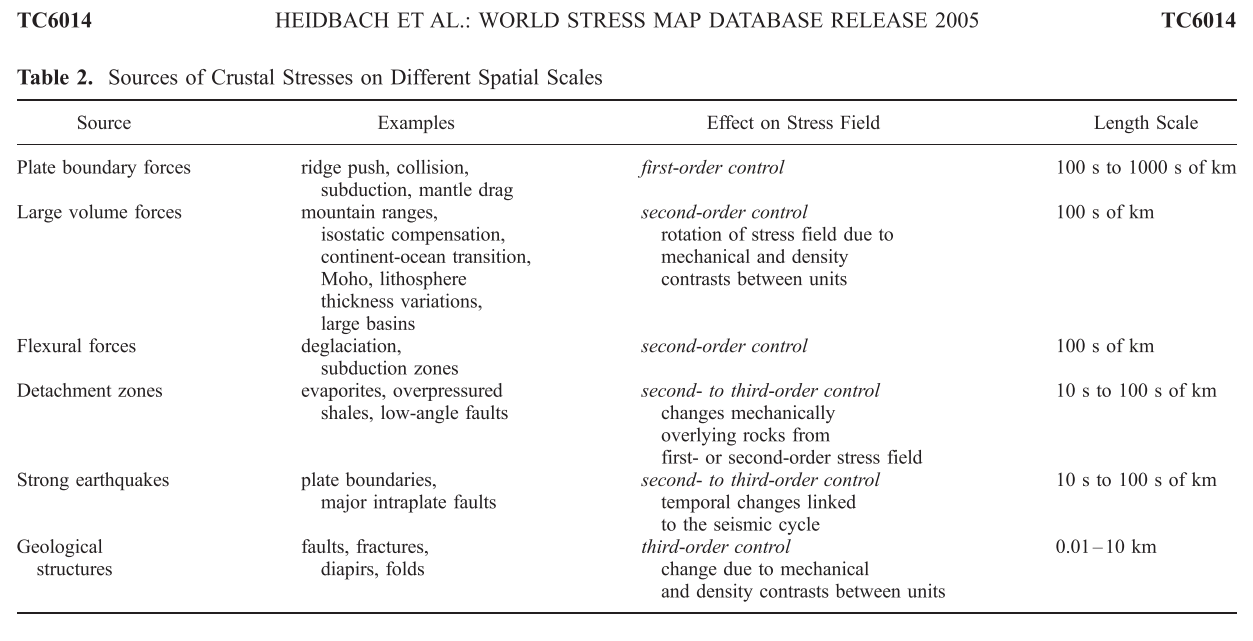
\includegraphics[width=\linewidth]{stress_sources.png}
      \tiny\textit{Heidbach et al. (2016)}
  \end{minipage}  
\end{frame}

 \begin{frame}{Link between plate motion and the orientation of stress tensor}
 \begin{minipage}{.4\linewidth}
 \small
  \begin{enumerate}[<+->]
    \item Strongest tectonic force(s) = plate boundary forces (Forsyth \& Uyeda, 1975): Plate boundary forces = source for most of the lithospheric stresses (e.g. Zoback \& Zoback 1989)
    \item $\sigma_\text{Hmax} \approx \sigma_\text{plate boundary}$
    \item Forces along trajectories of the plates’ relative motion (Forsyth \& Uyeda, 1975)
    \item Stress along trajectories of the plates’ torque and relative rotation (Wdowinski, 1999)
  \end{enumerate}
  \end{minipage}
  \hfill
  \begin{minipage}{.58\linewidth}
      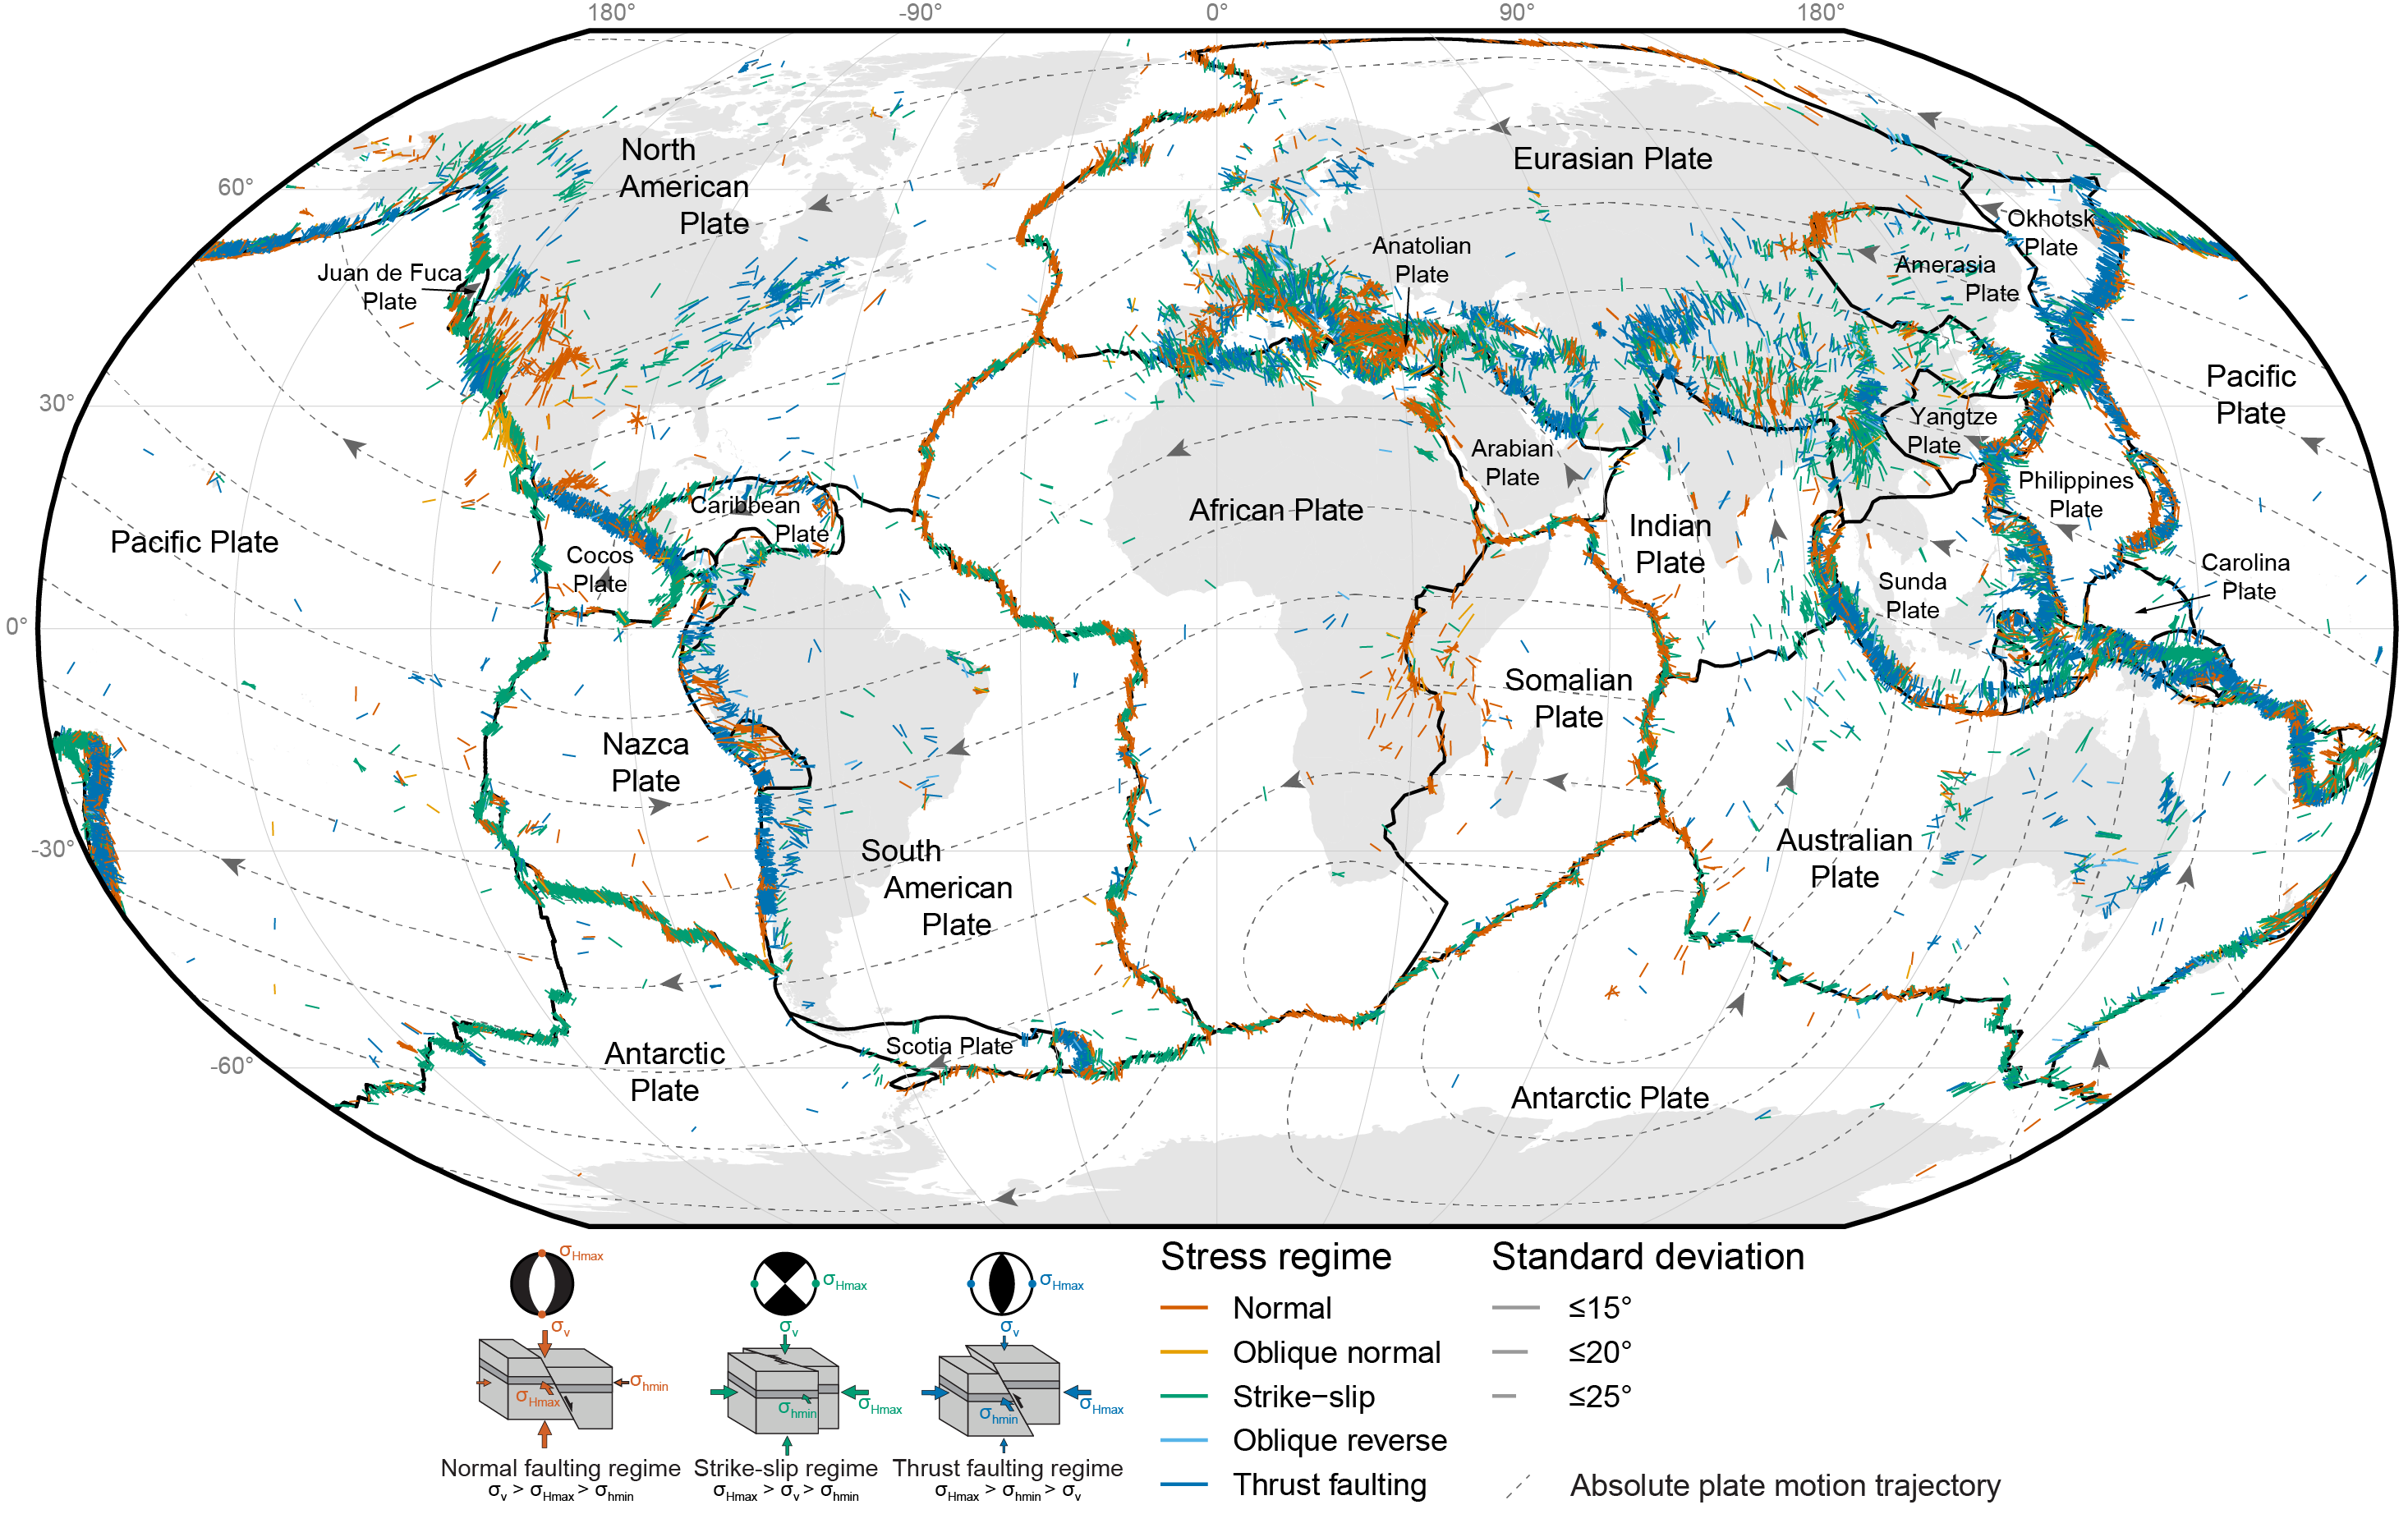
\includegraphics[width=\linewidth]{Figure_13_stress_world.png}
      \tiny\textit{Stephan et al. (2023)}
  \end{minipage}  
\end{frame}

  
\section{Plate motion}

	\begin{frame}{Plate motion on a sphere = rotation}{Geometrical analysis of plate motion}
	\begin{minipage}{.49\linewidth}
	\small
	  \begin{itemize}[<+->]
        \item Plate tectonics describe motion of lithospheric plates over the astenosphere
	    \item \textit{Spherical polygons rotate on the outer shell of a sphere}
	    \item Parametrization in terms of angle and axis
	    \item Rotation axis passes trough centre of Earth (\textbf{Euler pole})
	  \end{itemize}
	\end{minipage}
    \hfill
    \begin{minipage}{.49\linewidth}
    \centering
	\includegraphics<1->[height=.8\textheight]{euler_pole1.png}	
	%\includegraphics<2>[height=.825\textheight]{euler_pole.png}	
    \only<1->{\\ \tiny\textit{Cox \& Hart (1986)}}
    \end{minipage}	
	\end{frame}		
	
%%%%%%%%%%%%%%%%%%%%%%%%%%%%%%%%%%%%%%%%%%%%%%%%%%%%%%%%%%%%%%%%%%%%%%

	\begin{frame}{Horizontal stress at Earth´s surface}{Anderson´s Law}
	\begin{minipage}{.4\linewidth}
	  \begin{itemize}[<+->]
        \item Air has no shear stress
        \item Anderson (1951): At Earth´s surface the principal stress directions are directions of zero shear stress 
	    \item Earth´s surface = principal plane of stress, containing two of the principal stress directions
	    \item third principal stress direction is normal to the Earth's surface
	  \end{itemize}
	\end{minipage}
    \hfill
    \begin{minipage}{.59\linewidth}
    \centering	
	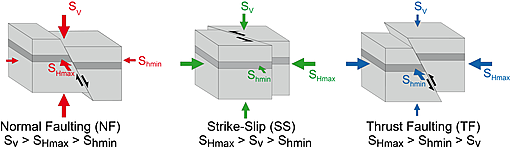
\includegraphics[width=\linewidth]{stress}	
	\tiny\textit{Sperner et al. (2014)}
    \end{minipage}	
	\end{frame}	
	
%%%%%%%%%%%%%%%%%%%%%%%%%%%%%%%%%%%%%%%%%%%%%%%%%%%%%%%%%%%%%%%%%%%%%%

\begin{frame}{Plate motion vs. horizontal stress (1)}
    \begin{minipage}[c][0pt][c]{.4\linewidth}
    \begin{itemize}
      \item Plate boundary forces (e.g. slab-pull, ridge push) control first-order intraplate deformation (\textit{Zoback et al. 1989})
      \item Max. horizontal stress ($\sigma_{Hmax}$) is parallel or perpendicular to relative plate motion direction (\textit{Wdowinski 1998})
    \end{itemize}    
    \end{minipage}
	\hfill
    \begin{minipage}[c][200pt][c]{.58\linewidth}	
	\centering		
    \only<1>{
        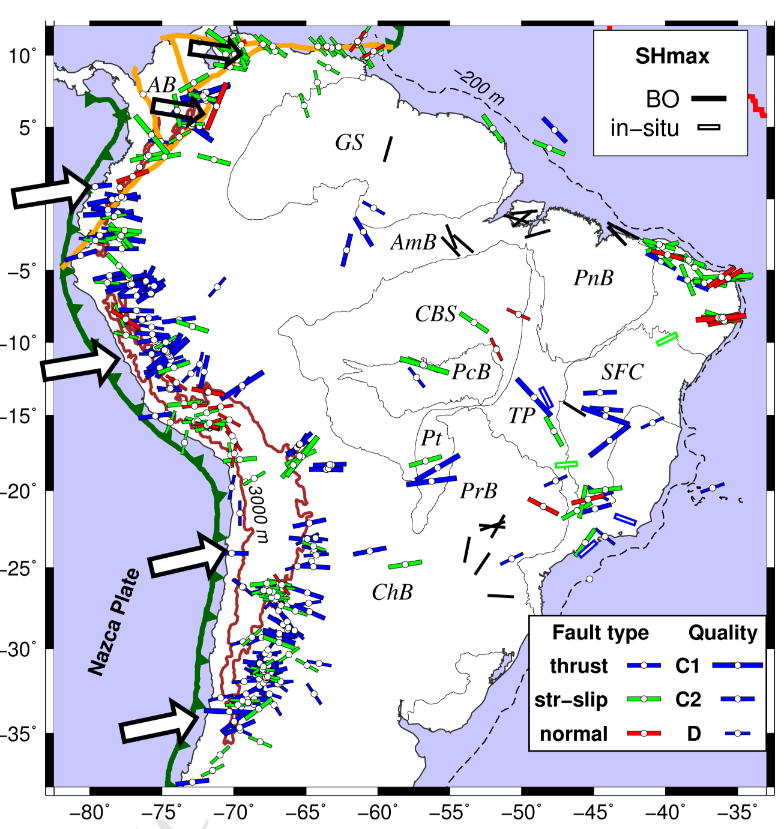
\includegraphics[height=.8\textheight]{sam.png}\\ 
        \tiny\textit{Assumpção et al. (2016)}
        }	
    \only<2>{Orientation of tectonic features relative to plate motion\\
        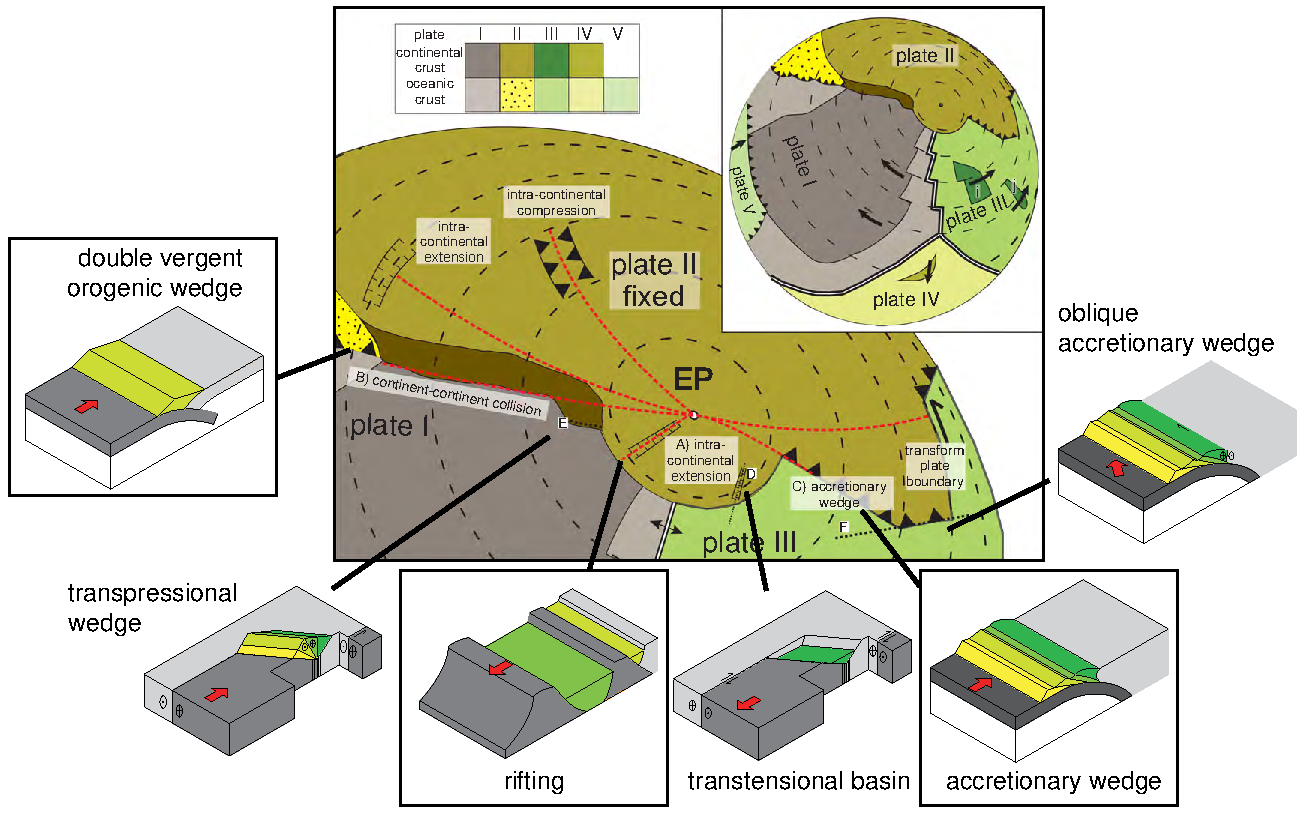
\includegraphics[width=\linewidth]{kroner2016.pdf}\\%
        \tiny\textit{Kroner et al. (2016)}
        }
    \end{minipage}    
	\end{frame}	
	
%%%%%%%%%%%%%%%%%%%%%%%%%%%%%%%%%%%%%%%%%%%%%%%%%%%%%%%%%%%%%%%%%%%%%%
% \subsection{Relative plate motion}	
% 	\begin{frame}{Reconstruction of relative plate motion}
% 	\begin{minipage}[c][0pt][c]{.4\linewidth}
% 	  \begin{itemize}[<+->]        
% 	     \item Great circles segments: e.g. spreading ridges, subduction zones
% 	     \item Small circle segments: transform fault, spreading rate, slip vectors, GPS
% 	     %\item Conversion between reference systems by \enquote{concatenation}, i.e. sequential composition of rotations
% 	   \end{itemize}
% 	\end{minipage}
% 	\hfill
%     \begin{minipage}[c][200pt][c]{.58\linewidth}		
%     \centering                
%         \only<1>{Orientation of tectonic features relative to plate motion\\
%         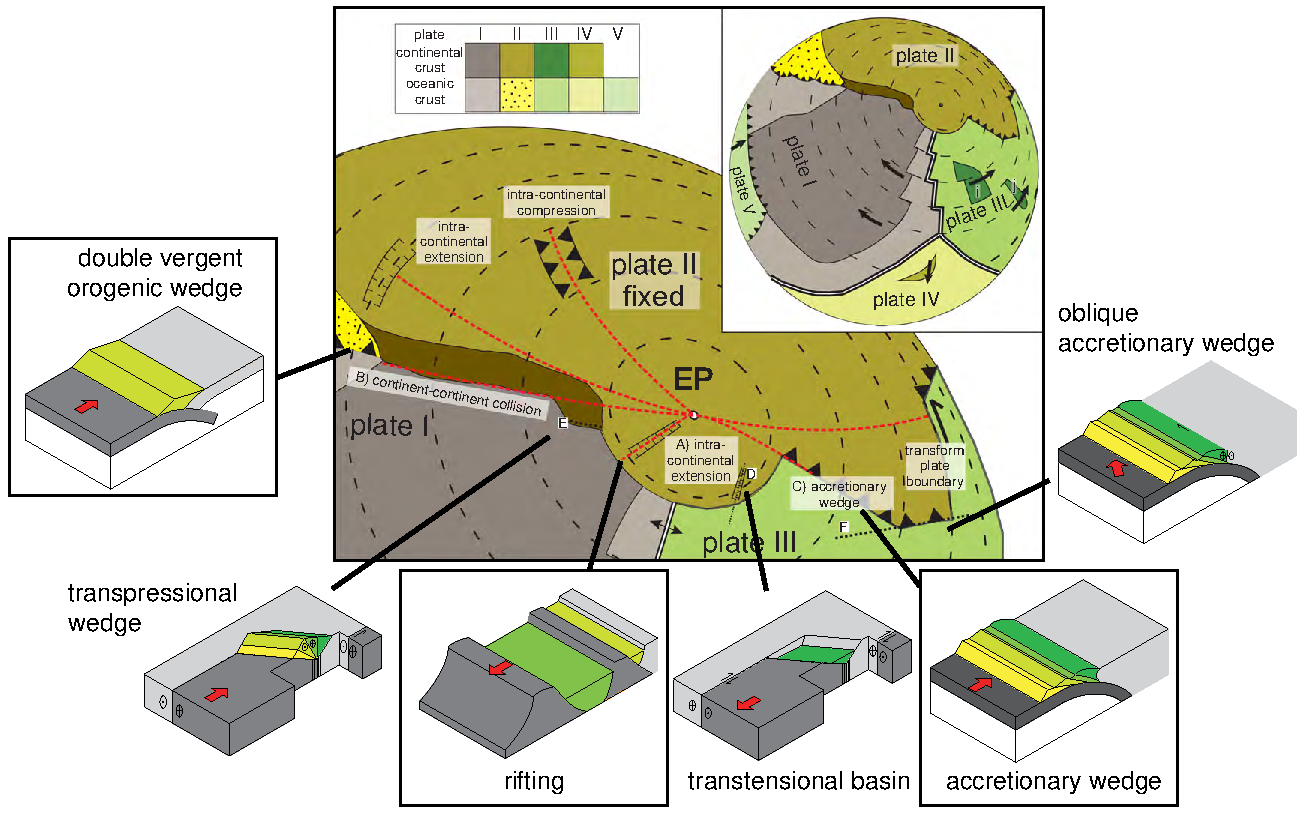
\includegraphics[width=\linewidth]{kroner2016.pdf}\\%
%         \tiny\textit{Kroner et al. (2016)}}
%         \only<2>{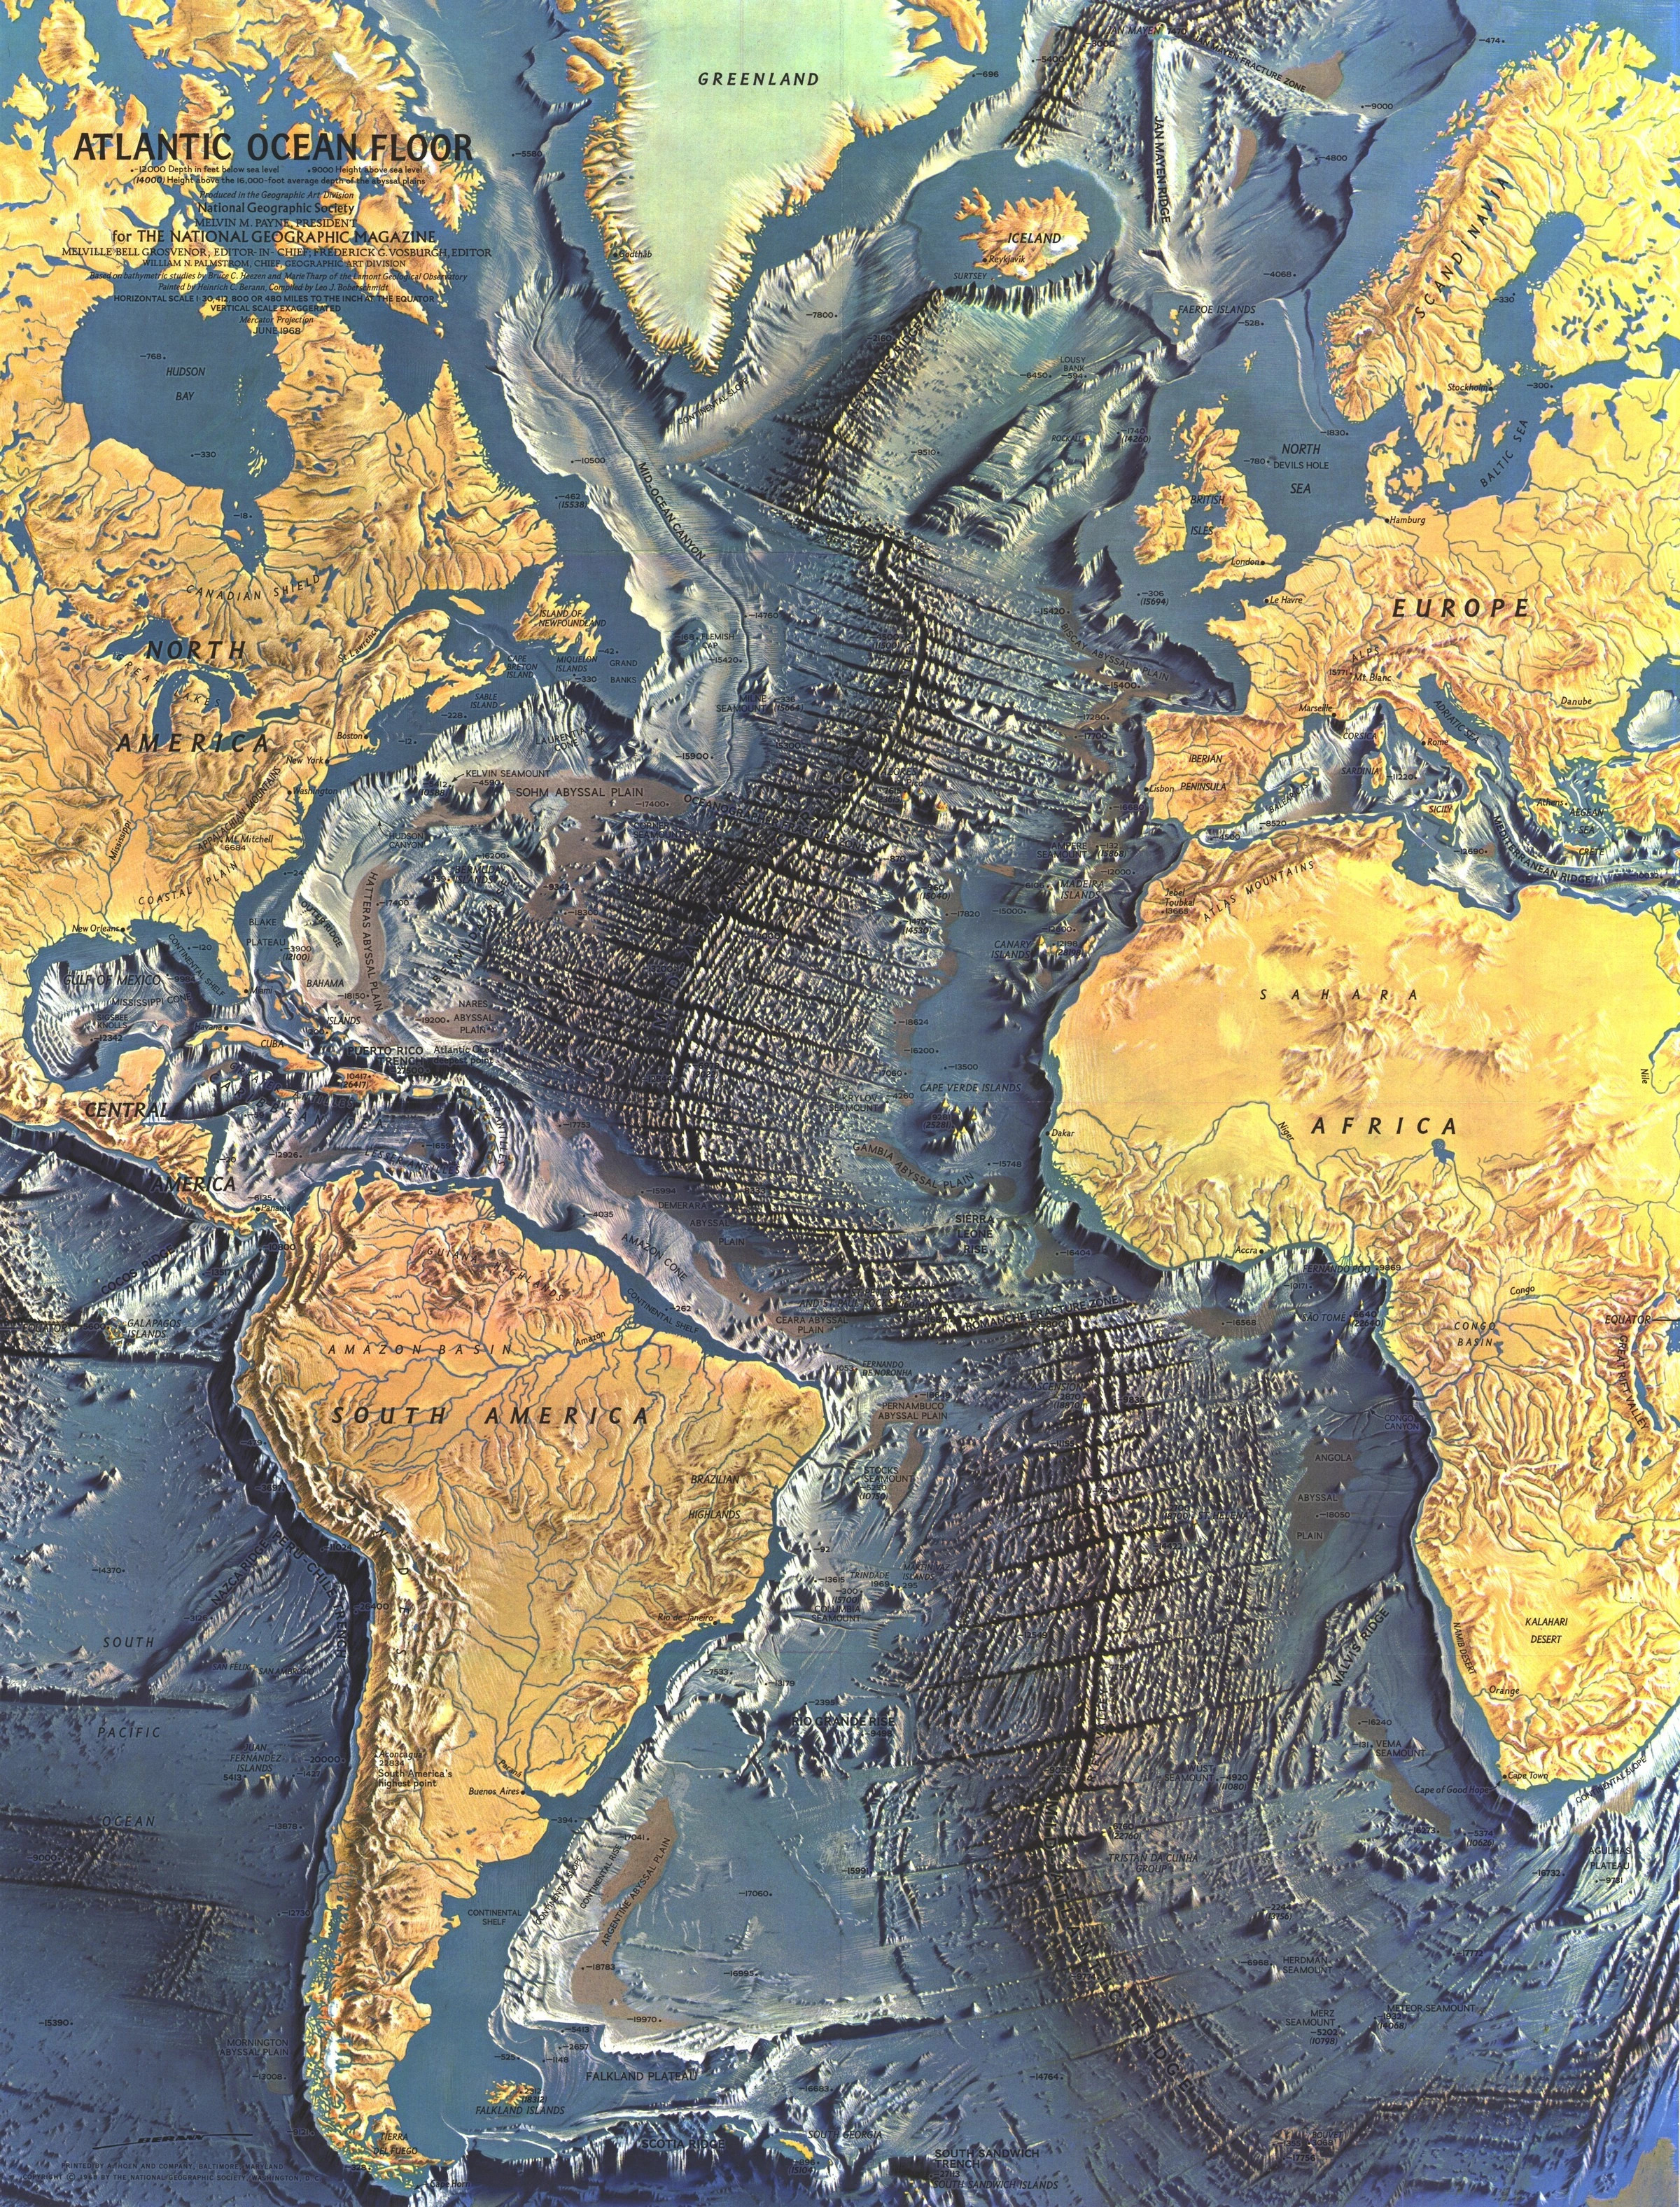
\includegraphics[height=.8\textheight]{atlantic}\hfill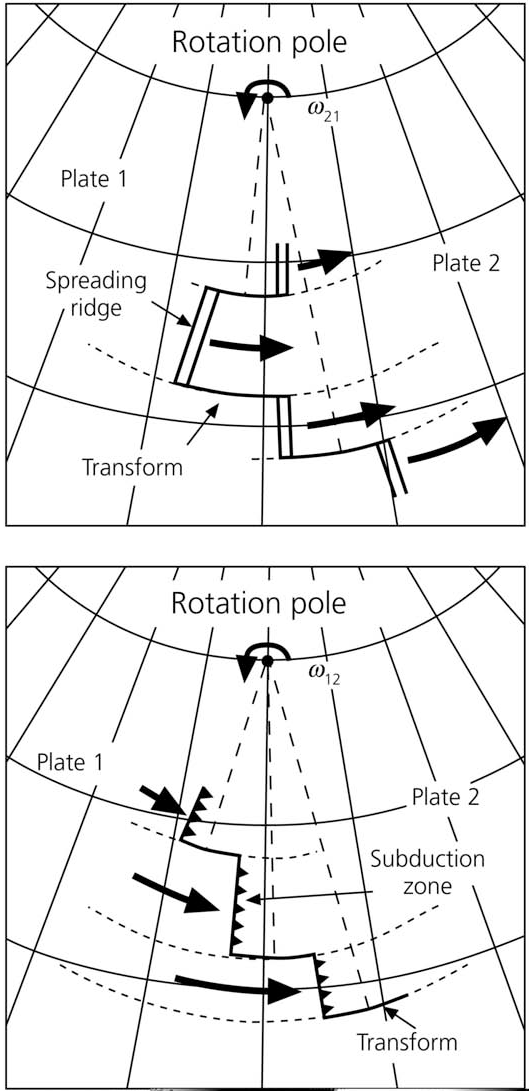
\includegraphics[height=.8\textheight]{stein1.png}}        
%         \only<3>{\includegraphics[height=.8\textheight]{sella_gps.png}\\
%         \tiny\textit{Sella et al. (2002)}}
%     \end{minipage}		
% 	\end{frame}
% 	
% %%%%%%%%%%%%%%%%%%%%%%%%%%%%%%%%%%%%%%%%%%%%%%%%%%%%%%%%%%%%%%%%%%%%%%
% \subsection{Absolute plate motion}
% 	\begin{frame}{Reference systems or what is kept fix}
% 		\begin{minipage}[c][200pt][c]{.42\linewidth}
% 		\begin{itemize}[<+->]
% 		\item All reference systems are virtual
% 		\item \textit{Relative plate motion}: one plate is fix (used for plate motion reconstruction)
% 		  \item \textit{Absolute plate motion}: motion relative to a fixed reference system (geodynamic meaning?)
%             \begin{itemize}
%                 \item Present: hot spots (mantle) vs. space geodesy (celestial sphere)
%                 \item Past: hot spots, paleomagnetism, and paleolatitudes (sedimentary facies, fossils...)	
%                 \end{itemize}
% 		\end{itemize}		 	  
% 		\end{minipage}
%         \hfill
%         \begin{minipage}[c][0pt][c]{.57\linewidth}
%         \centering
%             \includegraphics<1-2>[height=.825\textheight]{san-andreas}
%             %\includegraphics<1>[height=.825\textheight]{plate_circuit.png}
%             %    \only<1>{\newline \tiny\textit{DeMets et al. 1990}}
%            \only<3>{Global absolute plate motions from space geodesy}
%             \includegraphics<3>[width=\linewidth]{C:/Users/tobis/FAUbox/Austausch/euler_pole-theory/small_circles/mollweide_bw.pdf}
%                 \only<3>{\newline \tiny\textit{after Sella et al., 2002)}}
%             \includegraphics<4>[width=\linewidth]{hot_spots.png}   
%             \only<5>{
%                 \begin{minipage}{.4\linewidth}
%                   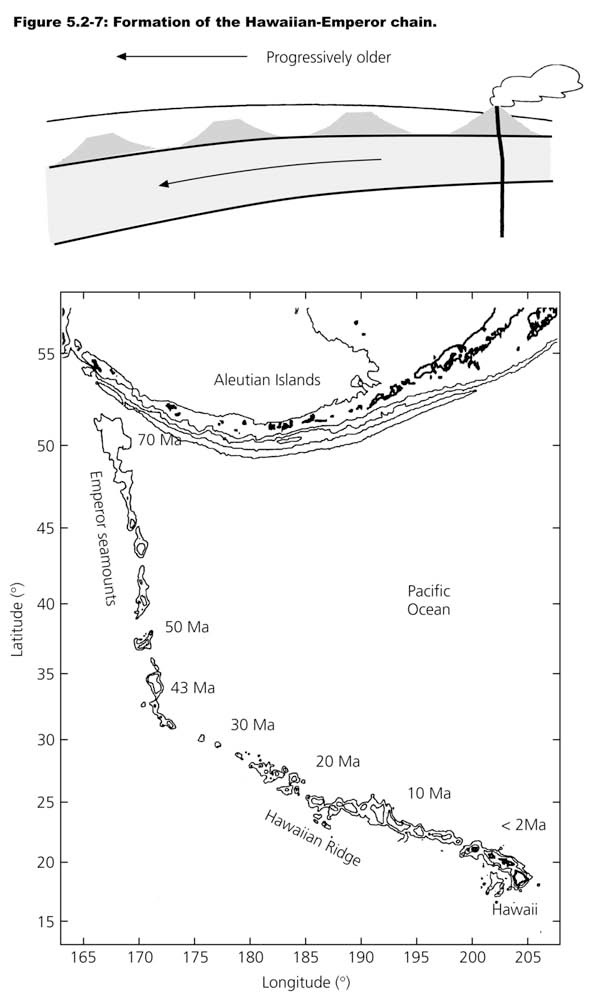
\includegraphics[width=\linewidth]{hawaii.png}
%                 \end{minipage}
%                 \hfill
%                 \begin{minipage}{.58\linewidth}
%                 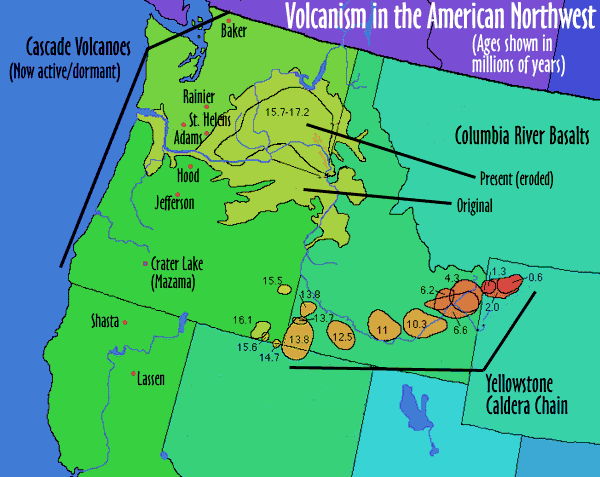
\includegraphics[width=\linewidth]{yellowstone.png} 
%                 \end{minipage}
%             }
%             %\includegraphics<6>[height=.825\textheight]{hawaii2.png}
% 		\end{minipage}
% 	\end{frame}
	
%%%%%%%%%%%%%%%%%%%%%%%%%%%%%%%%%%%%%%%%%%%%%%%%%%%%%%%%%%%%%%%%%%%%%%
\subsection{Link between plate motion and first-order stress}
\begin{frame}{Plate motion vs. horizontal stress (2)}{Rigid plates concept}
    \begin{minipage}[c][0pt][c]{.4\linewidth}
        \begin{itemize}[<+->]\small
            \item Assumption: rigid plates, i.e. \textbf{entire} deformation is accumulated along plate boundaries
            \item Diffuse plate boundaries and far-field stress????    
            \item How is the stress transferred to the plate´s interior?
            \item Additional processes controlling the orientation of intraplate stress?
        \end{itemize}
        \end{minipage}
        \hfill
        \begin{minipage}[c][200pt][c]{.59\linewidth}
        \centering
            \only<1>{Global earthquake distribution\\
            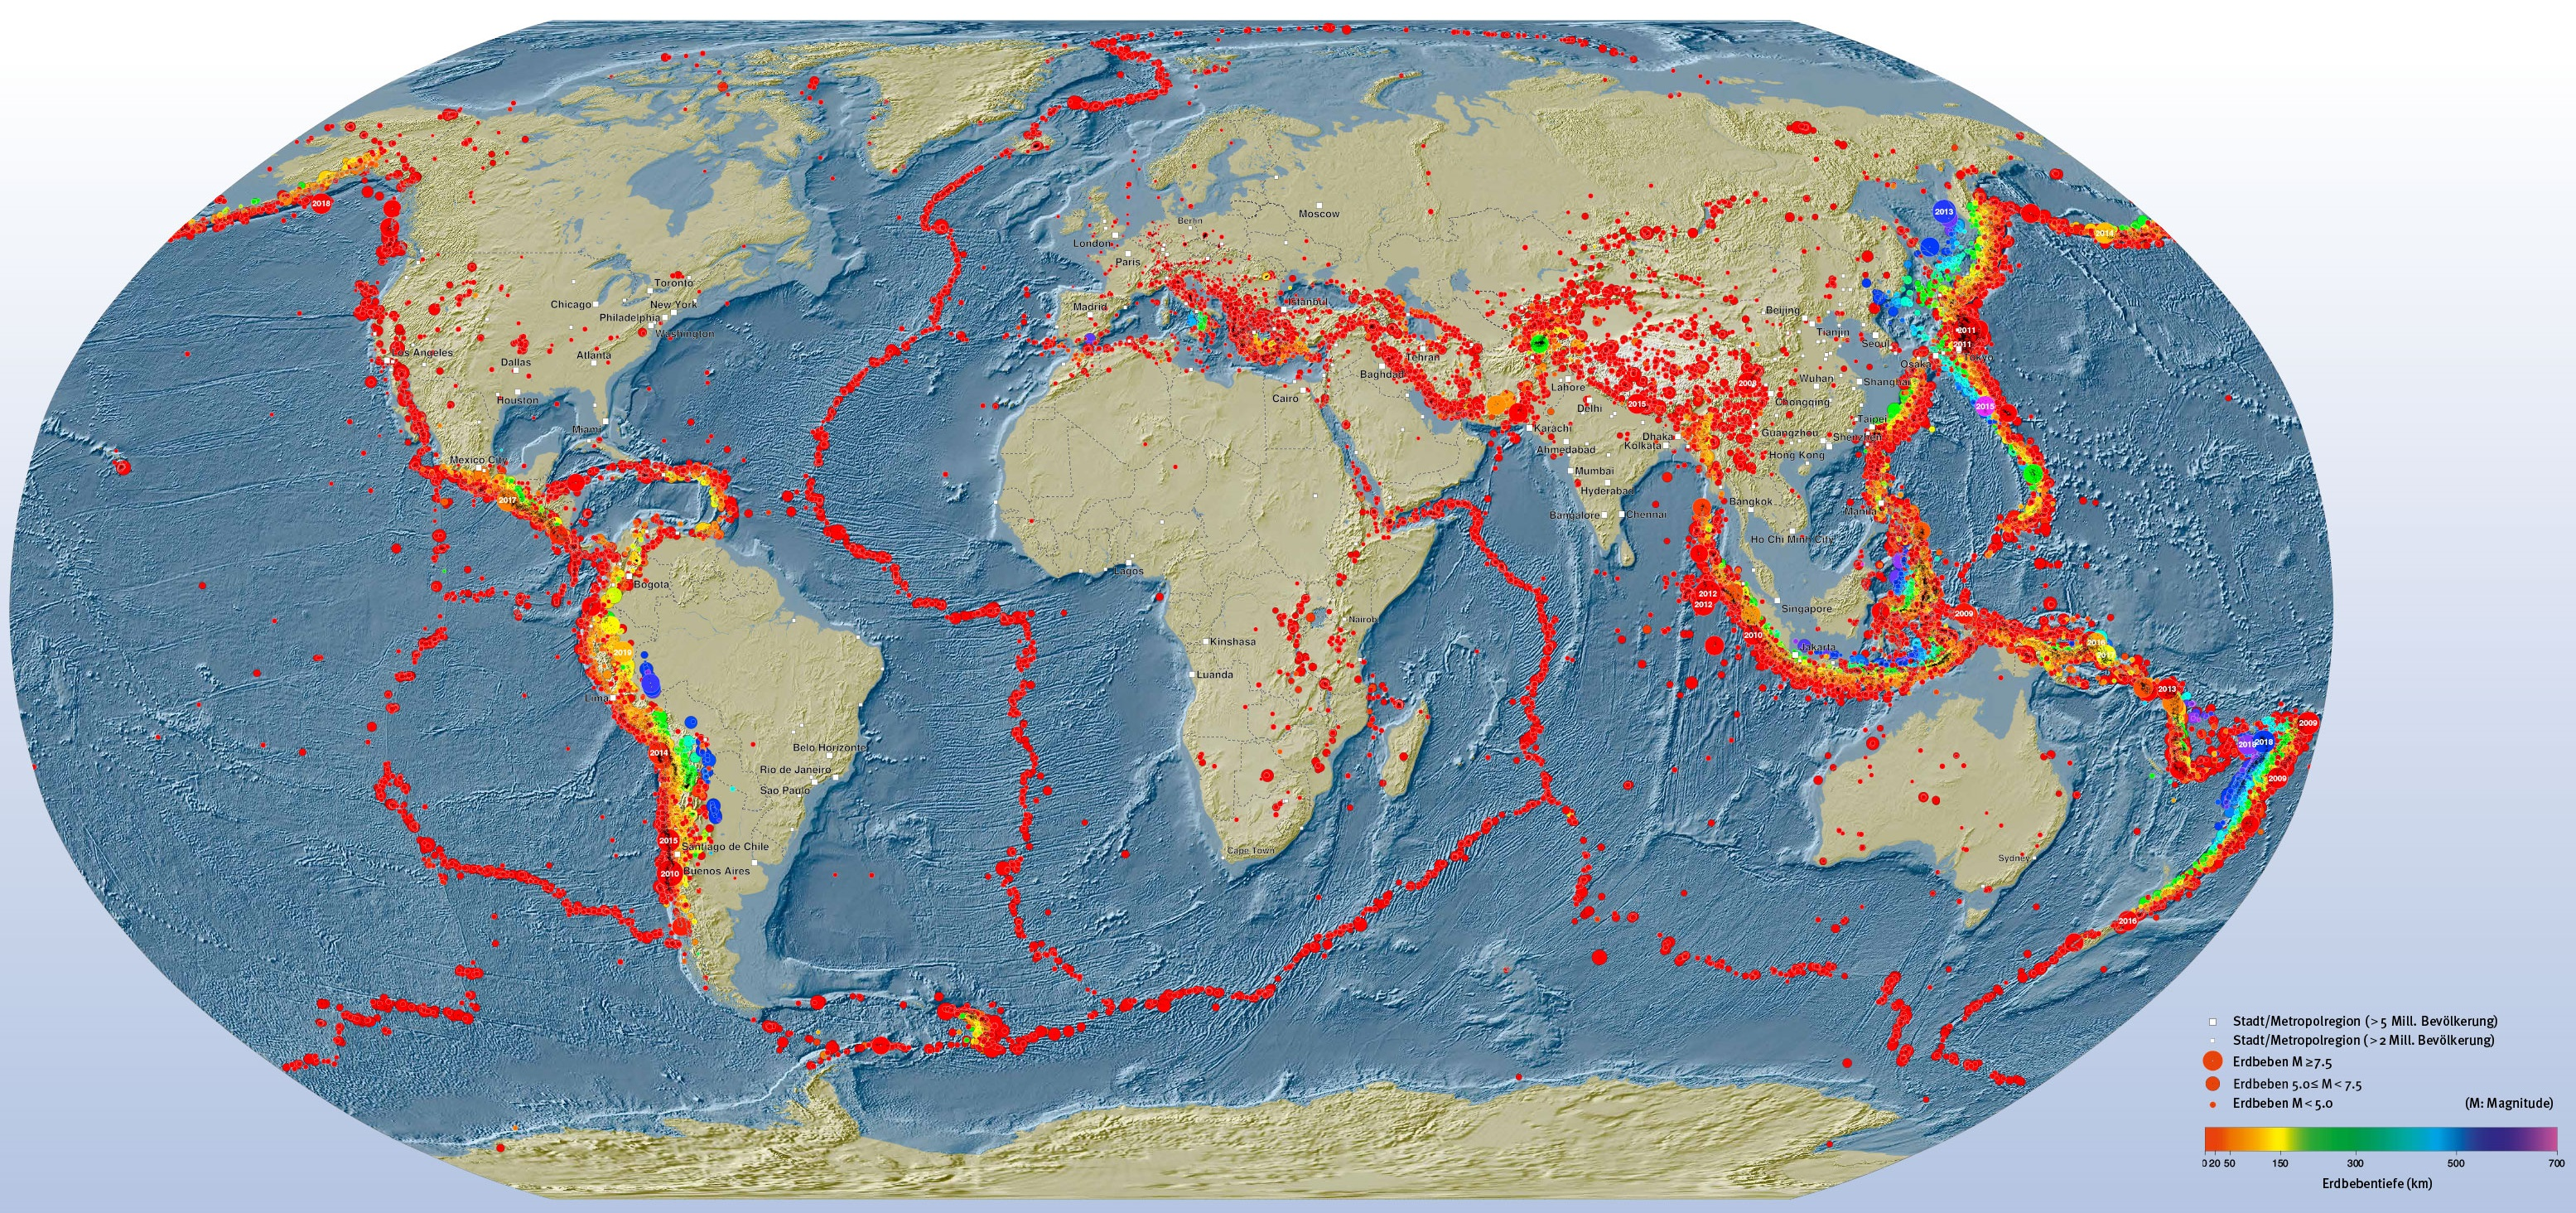
\includegraphics[width=\linewidth]{earthquakes.jpg}\\
            \tiny\textit{GFZ Potsdam}}
              
            \only<2->{Global crustal present-day stress field\\
            \includegraphics[width=\linewidth]{World_Stress_Map_2016_small.jpg}\\ 
            \tiny\textit{World Stress Map Project 2016}}
        \end{minipage}
	\end{frame}
  
  
\section{Method}
%------------------------------------------------
   
\begin{frame}{Method}{Quantifying the link between plate motion and first-order stress}
    \begin{minipage}{.6\linewidth}
    \small
        \begin{enumerate}[<+->]   
        \item Infer relative motion from absolute motions or other relative motions (compositions of rotations)
            \begin{itemize}
              \item Present day: calculate equivalent rotations (i.e. the motion between the fixed plate (where the deformation happens) and the colliding/diverging plate)
              \item Past: intermediate, equivalent rotation of plate motion history
            \end{itemize}
        \item Calculate the plate motion vector (trajectory) at coordinates of interest (azimuth of great circle direction between the resulting Euler pole and a given location)
        \item Calculate angular difference between the plate motion trajectories and the (paleo-) $\sigma_{Hmax}$ direction 
       \end{enumerate}
    \end{minipage}
    \hfill
    \begin{minipage}{.39\linewidth}
    \centering
	%\includegraphics<1>[width=\linewidth]{C:/Users/tobis/FAUbox/LfU-Projekt Störungsinventar (Harald Stollhofen)/Reports/Projekt Störungskataster/figures/stephan/plates_84Ma.pdf}
	\only<1>{%
            \animategraphics[loop, controls, autoplay, width=\linewidth]{5}{animation1/image_}{01}{36}%
	}%
	\only<2>{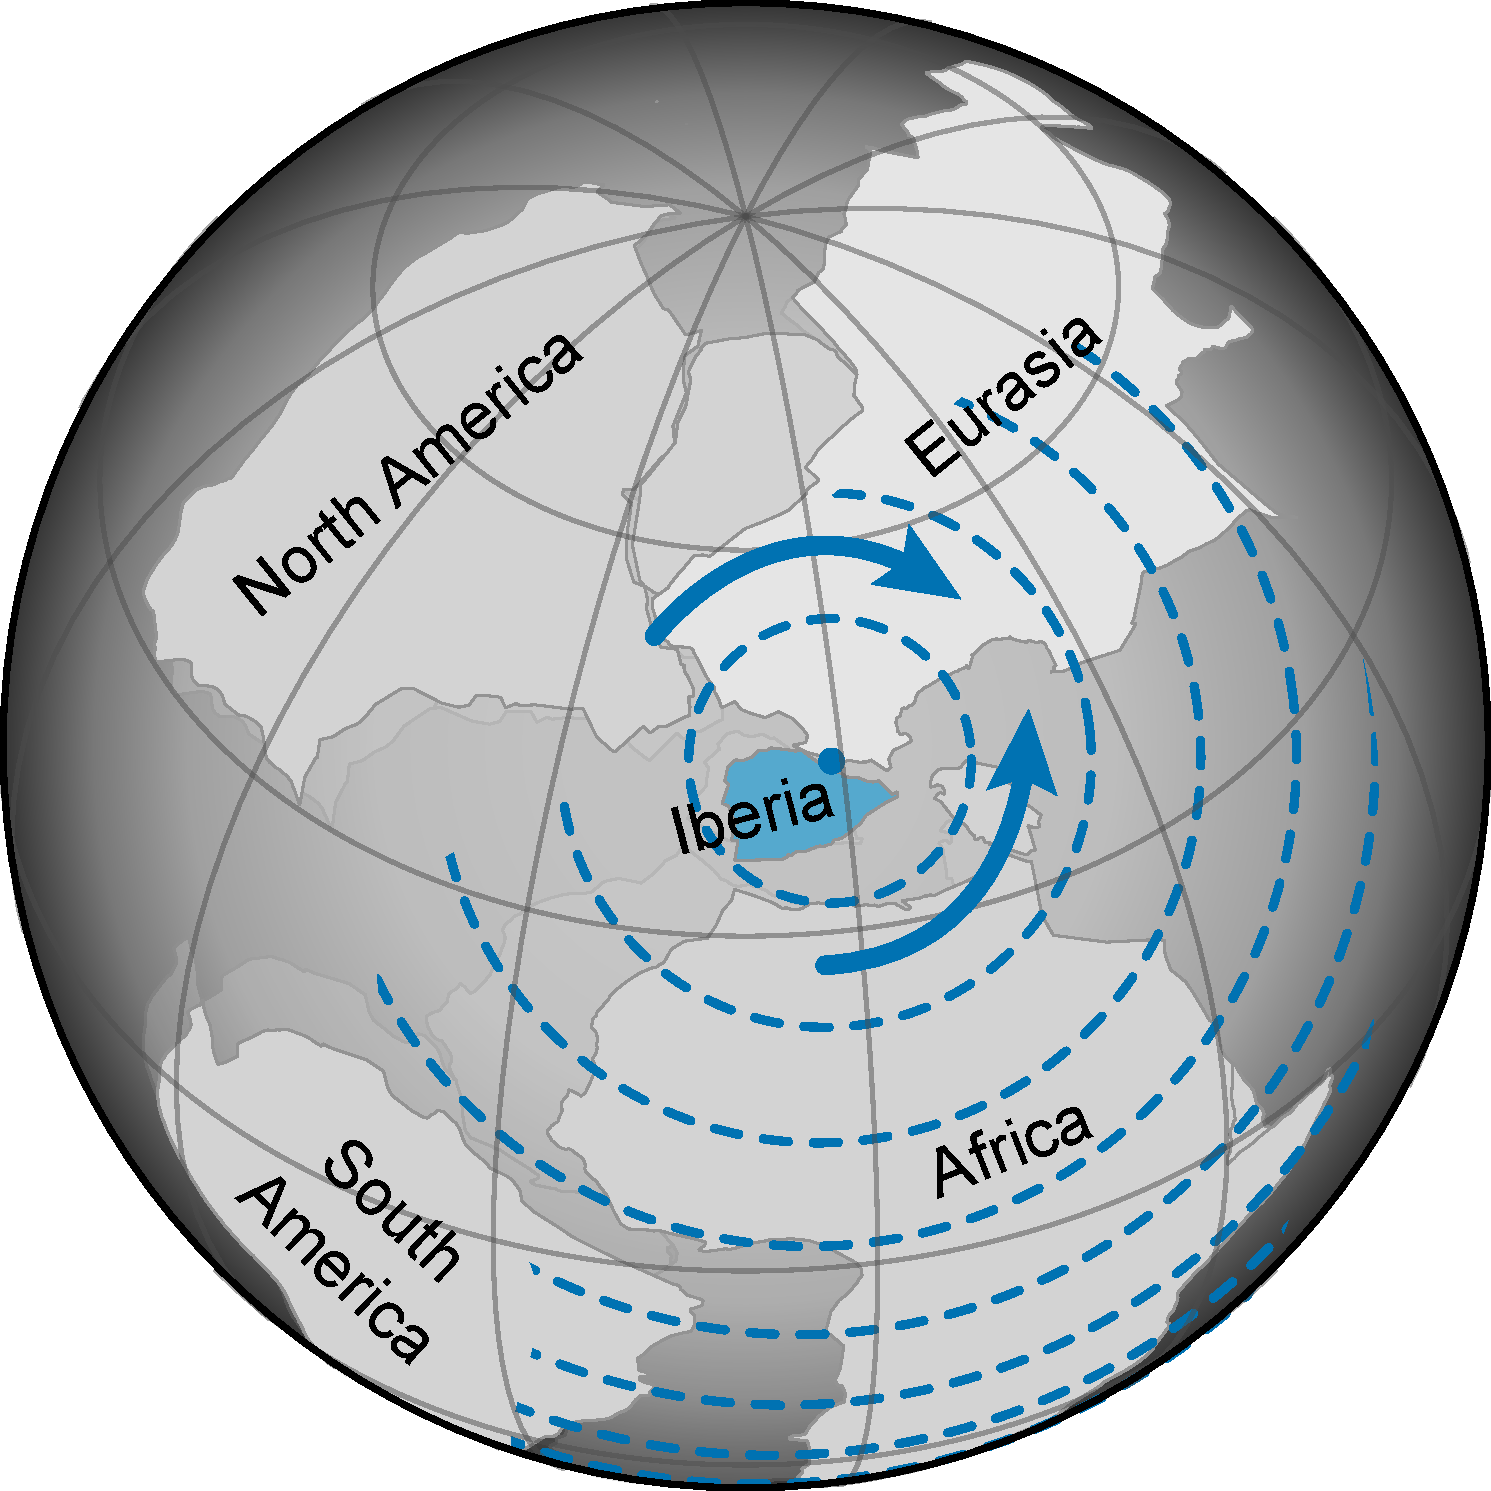
\includegraphics[width=\linewidth]{plates_84Ma.pdf}}%
	\only<3>{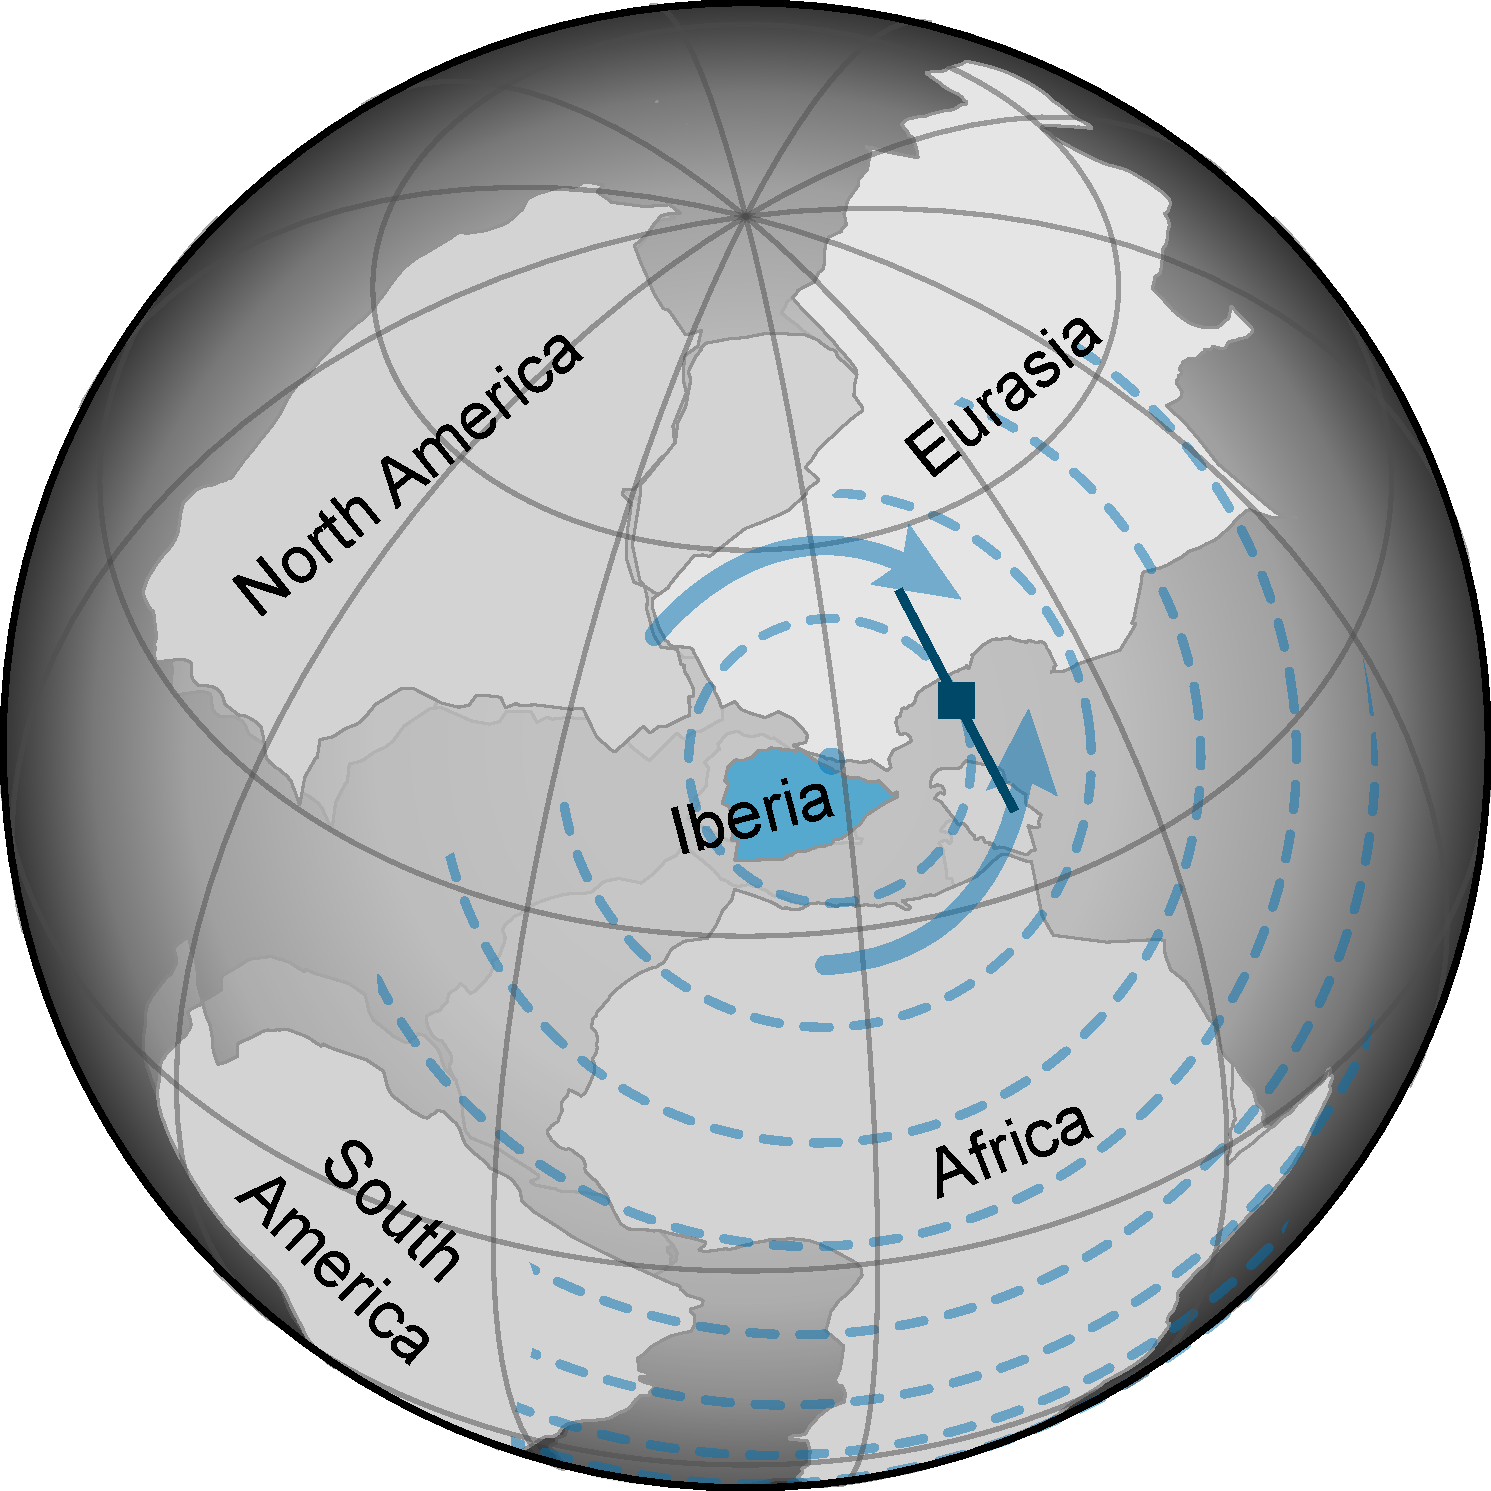
\includegraphics[width=\linewidth]{plates_84Ma_2.pdf}}%
	\only<4>{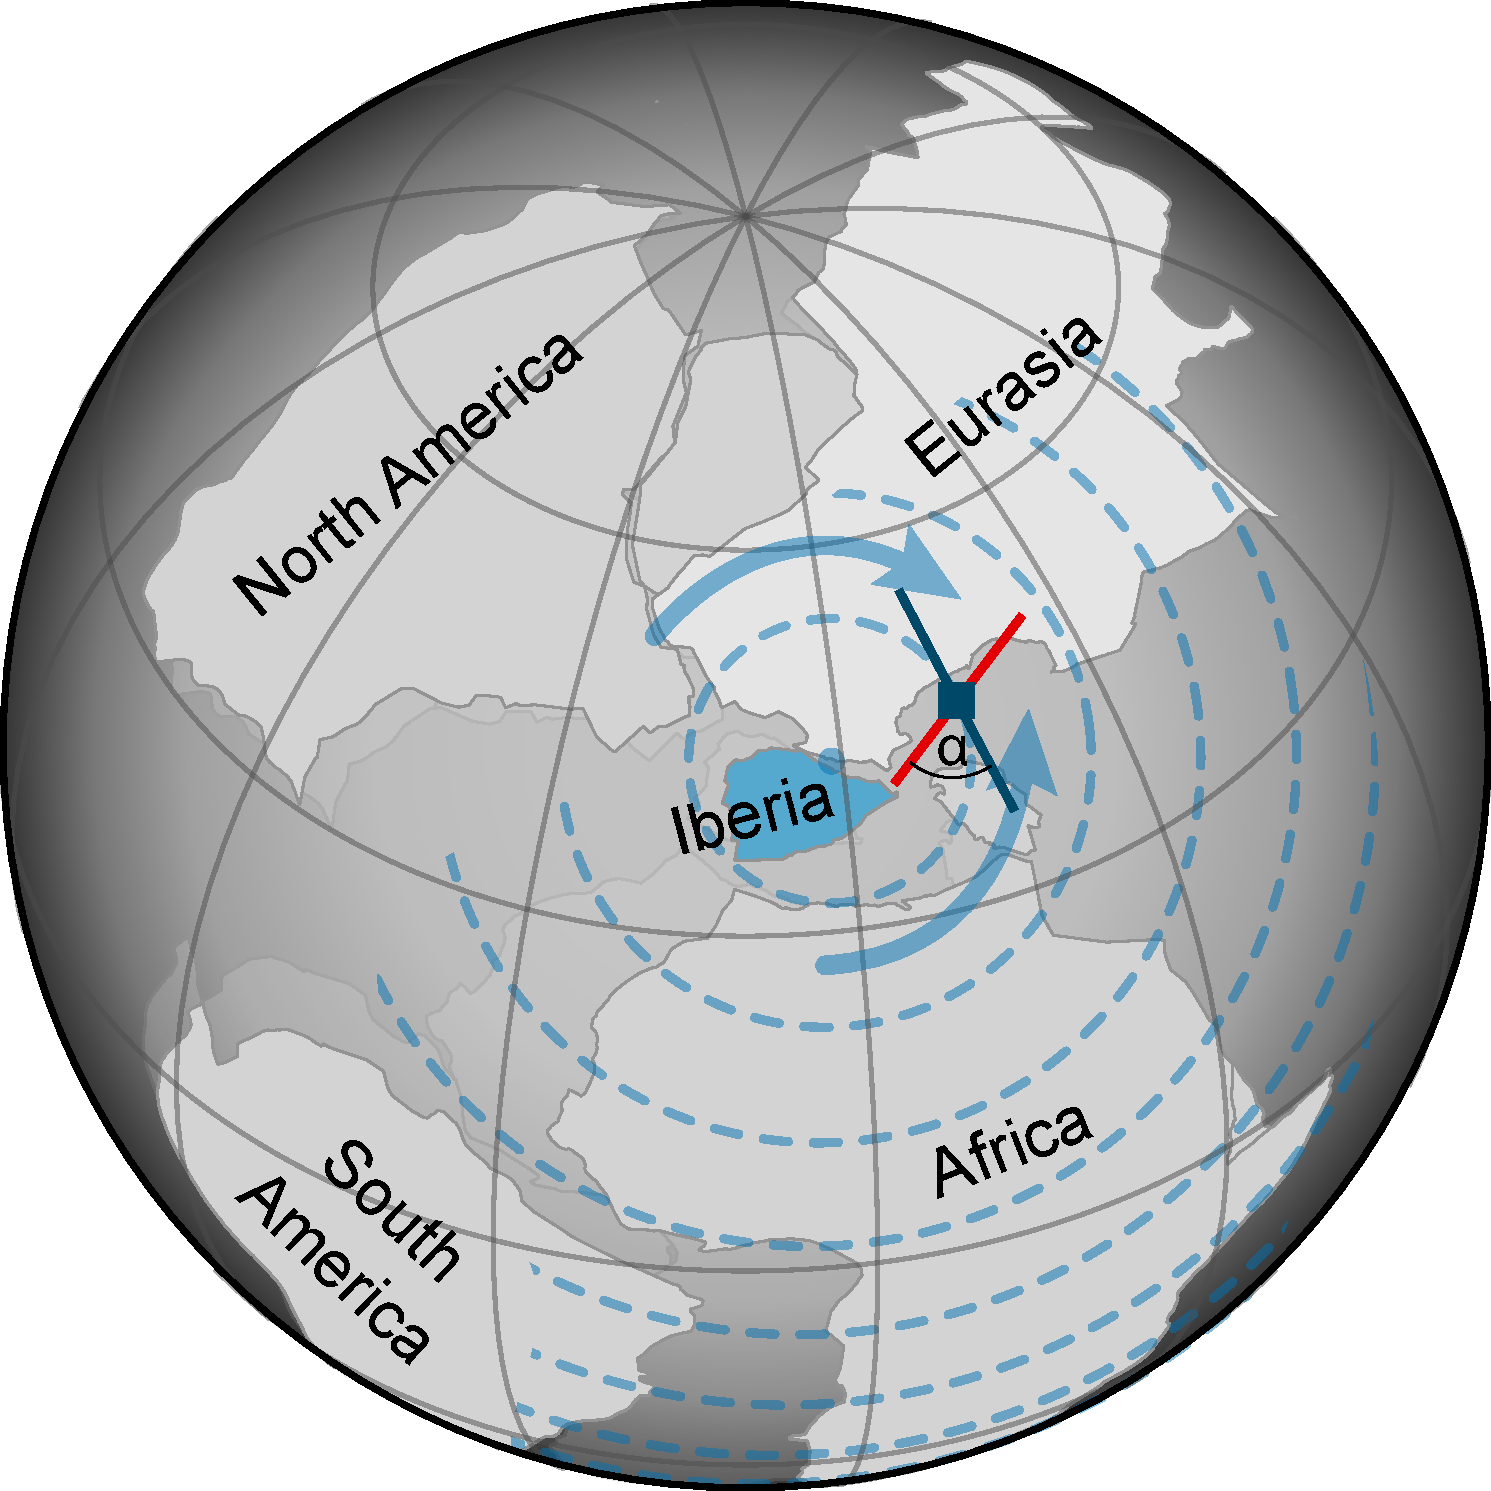
\includegraphics[width=\linewidth]{plates_84Ma_3.pdf}}%
    \end{minipage}
    \end{frame}
 
 \begin{frame}{Method}{Geometrical concept}
 \begin{minipage}{.54\linewidth}
   %\small 
   \[
    \sin\theta = \frac{\sin{\Delta\phi} \; \sin{(90^\circ - \lambda_\text{PoR})}}{\sin{\gamma}} =
     \frac{\sin{\Delta\phi} \; \cos{\lambda_\text{PoR}}}{\sin{\gamma}}
 \]
 \end{minipage}
 \hfill
 \begin{minipage}{.44\linewidth}
   %\includegraphics<1>[height=.85\textheight]{Figure_05_euler_circles}
   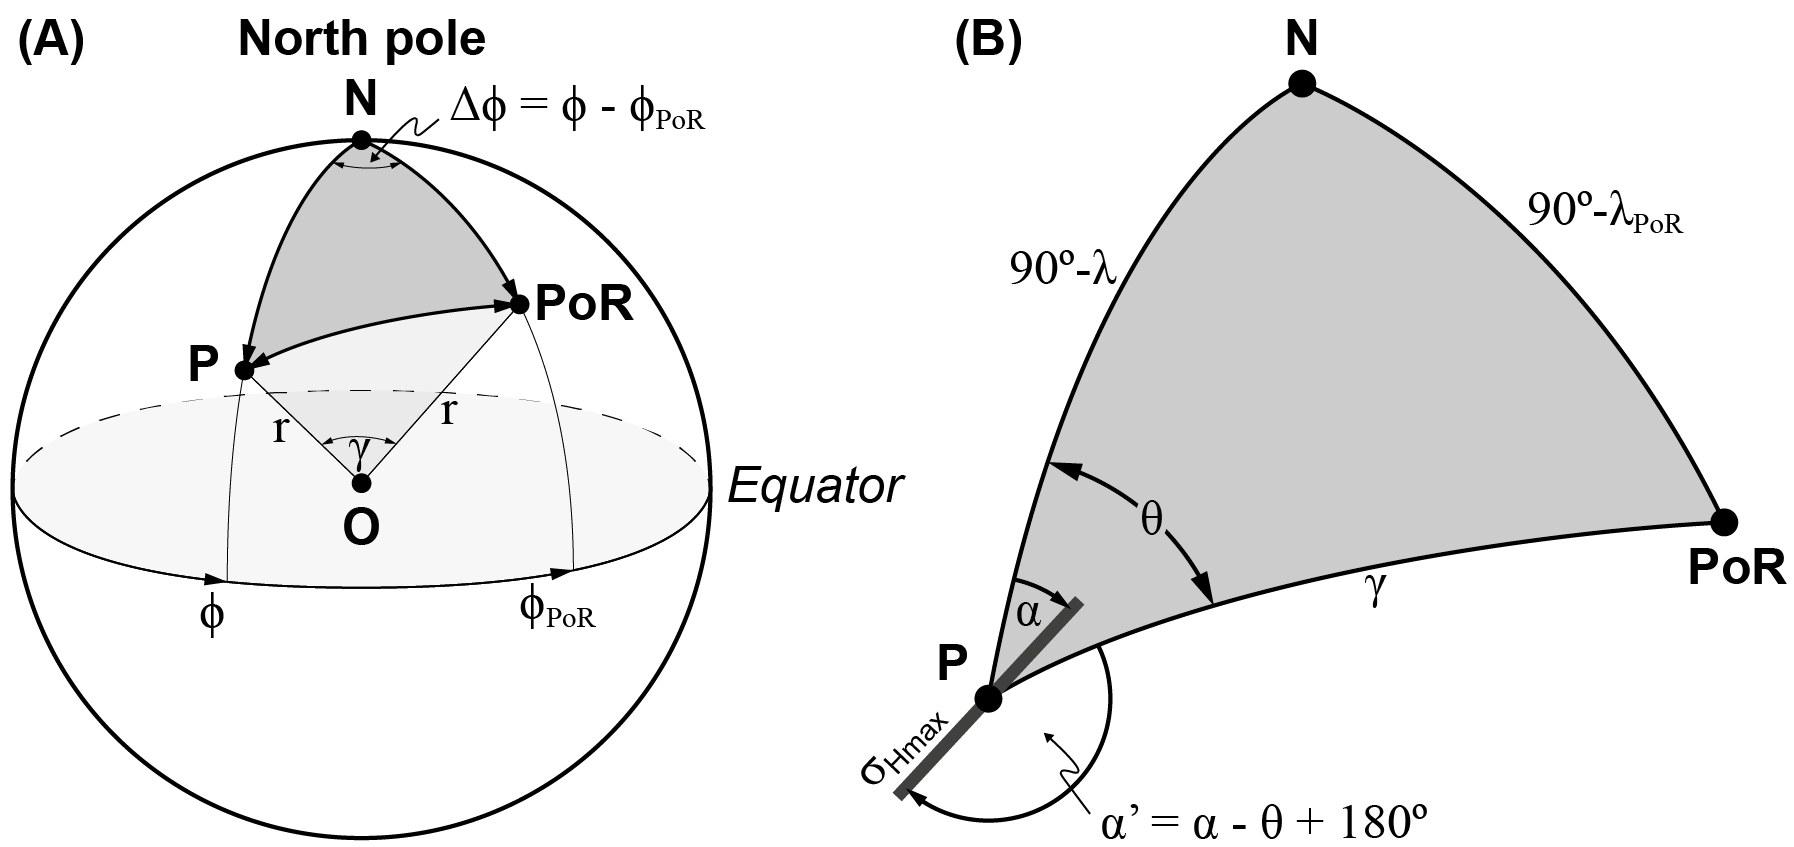
\includegraphics[width=\linewidth]{Figure_06_spherical_triangle}
 \end{minipage}  
 
  \vfill
 
 \scriptsize
 Predicted azimuth ($\beta$) of maximum horizontal stress (\shmax{}) adjacent to the various plate boundary types in the geographical coordinate reference system.
 %\begin{table}[ht]    
  \begin{tabular}{llll}
    \toprule
    Displacement of plate boundary & Stress regime & \shmax{} azimuth & Geometry of trajectories \\
    \midrule
    Outward & normal fault & $\beta = \theta$ & great circles \\
    Tangential (L) & strike-slip (L) & $\beta = \theta + 45^{\circ}$ & counterclockwise loxodromes\\
    Inward & thrust & $\beta = \theta + 90^{\circ}$  & small circles\\
    Tangential (R) & strike-slip (R) & $\beta = \theta + 135^{\circ}$ & clockwise loxodromes\\
    \bottomrule
    \end{tabular}
    
   
    \tiny The minimum horizontal stress is perpendicular to $\beta$. Hence, it follows the trajectories perpendicular to those predicted for \shmax{}. \newline
    Abbreviations: L -- left-lateral, R -- right-lateral.
 %\end{table}
 %\end{minipage}
  
 
 \end{frame}

 
 
 \section{Application}
  \begin{frame}{Application}{San Andreas Fault -- Gulf of California}
   \centering
             \includegraphics<1>[height=.825\textheight]{san-andreas}
             \includegraphics<2>[height=.825\textheight]{Figure_07_san_andreas_data}
             \includegraphics<3>[height=.825\textheight]{Figure_08_san_andreas_anomaly_map}
 \end{frame}
 
 \begin{frame}{Application}{Alaska -- Canadian Cordillera}
   \centering
             \includegraphics<1>[width=\linewidth]{Alaska_stress}
             \includegraphics<2>[height=.825\textheight]{Alaska_other_models}
 \end{frame}
 
  \begin{frame}{Application}{Plate boundaries}
     \centering 
     \includegraphics<1>[height=.825\textheight]{Figure_13_stress_world}
     \includegraphics<2>[height=.825\textheight]{Figure_14_nchisq_world}
 \end{frame}
 
 \section{Short course}
  \begin{frame}{Outline short course}{}
   \begin{itemize}
     \item Circular statistics for orientation data
     \item Plate motion concepts (TS, UK) and mathematics (HS)     
     \item Link between plate motion and stress/strain (UK)
     \item Stress field analysis
     \item Lineament analysis \ldots
   \end{itemize}  
   
   \vfill
   \hrule
   \vfill
   
   Additionally: R, GIS
 \end{frame}

  
\end{document}
